\chapter{Auswertung}

\section{Kalibrierung}
Um den Totalreflexionswinkel zu bestimmen haben wir f�r verschiedene Wellenl�ngen von 500nm - 600nm 
einen gro�en Winkel zwischen 0 und 90 Grad bzgl des einfallenden Lichtstrahles abgefahren und die Reflexivit�t
des Glasprismas unter diesem Winkel gemessen.

Wir erwarten einen stufenf�rmigen Verlauf wobei die Reflexivit�t bei 0 anf�ngt, an dem Totalreflexionswinkel
auf 1 springt und bis 90 Grad weiterverl�uft. 

\begin{equation}
 \theta_{tot}=arcsin{\sqrt{\frac{\eps_{Luft}}{\eps_{Glas}(\lambda)}}}
\end{equation}

Dies ist eine idealisierte Betrachtungsweise. Wir werden im Experiment eine stetige Kurve an der Totalreflexionsstelle sehen
und versuchen f�r jeden Messdurchlauf diese Stelle mit 2 Geraden anzufitten.


Wie man im Bild xx sehen kann, verschiebt sich die Kurve bei h�heren Wellenl�ngen in Richtung gr��eren Winkeln, dies h�ngt mit 
der Frequenzabh�ngigkeit der Permitivit�t von Glas $\eps_{Glas}(\lambda)$ zusammen.

\begin{figure}[h]
    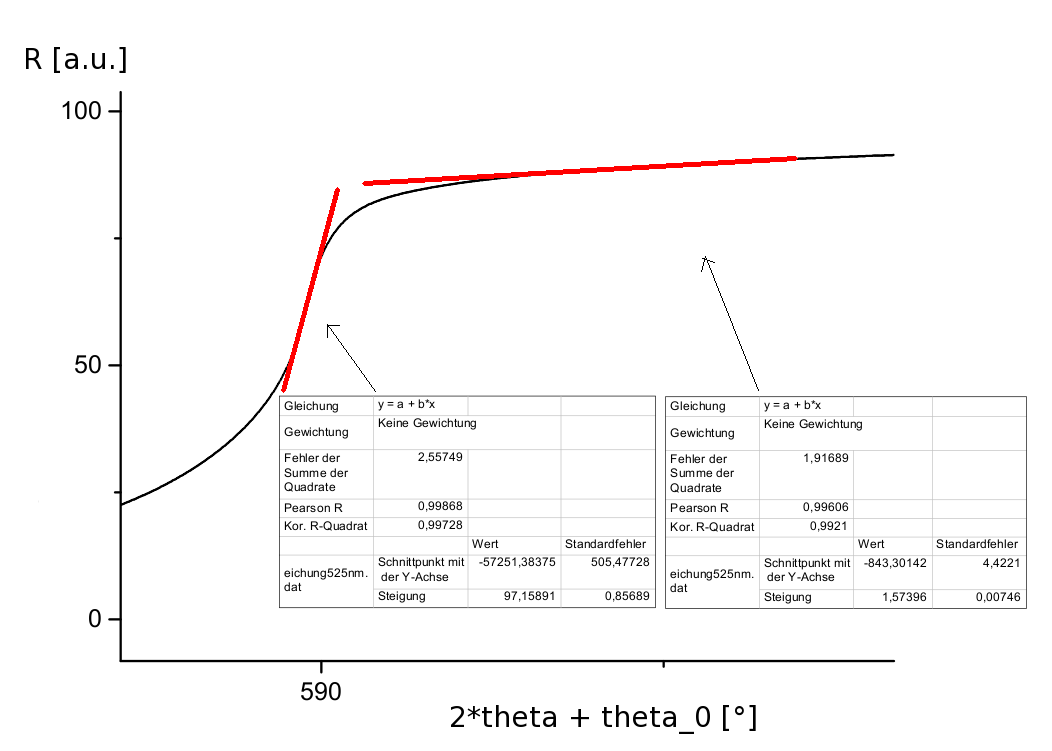
\includegraphics[width=1\textwidth]{linreg-totref-525nm.png}
	\caption{Gemessene Reflektivit�t $R$ in Abh�ngigkeit der zu kalibrierenden Winkelangabe
				des Rotationstisches $2\theta+\theta_0$. In Rot die linearen Regressionen
				zur Bestimmung des Totalreflexionswinkels.}
	\label{fig:linreg}
\end{figure}

Hier sieht man ein Beispiel f�r den Fit den wir an allen 5 Kurven durchgef�hrt haben. In der Tabelle xx sehen Sie nun
die eingestellten Wellenl�ngen, den theoretischen $\theta_{tot}$ und experimentellen Wert $\alpha_{tot}$  f�r die Totalreflexion, 
sowie den errechneten Offset $\theta_{0}$.

\begin{tabular}[t]{|l|l|l|l|}
\hline
$\lambda$ & $\theta_{tot}$ & $\alpha_{tot}$ &$\theta_{0}$ \\
\hline
Platz A & Wavetek Mod. 192, 20 MHz & Agilent Technologies DSO1002A\\
blaue Platine & & 60 MHz, Analog: Philips PM 3305\\
\hline
Platz B & HP 8111A, 20 MHz&  Tektronix TDS 2014C, 100 MHz\\
braune Platine & & \\
\hline
\end{tabular}

Wir beziehen uns hier auf \eqref{eq:r012}